\subsubsection{Statistics}
A user should be able to view statistics,
\begin{itemize}
	\item from and to a certain date
	\item for projects with a specific status
	\item for projects done by a specific author or co-author
	\item from which authors collaborated on projects
	\item based on the venue of a project(s)\\
\end{itemize}
More than one criteria should be able to be specified in other words you should be able for example view what the status is of all projects done by a certain author or co-author in a time period.\\ \\
\textbf{Pre-Conditions}
\begin{itemize}
	\item The user should be logged into UPRM.
	\item The user must be a administrator or general user. The user may not be a third party user.
	\item The user must have the right privileges to view the specific data.\\
\end{itemize}
\textbf{Post-Conditions}
\begin{itemize}
	\item Statistics should be displayed in a formatted table with headings.\\
\end{itemize}
\textbf{Statistics Use Case Diagram:}\\
\centerline{\fbox{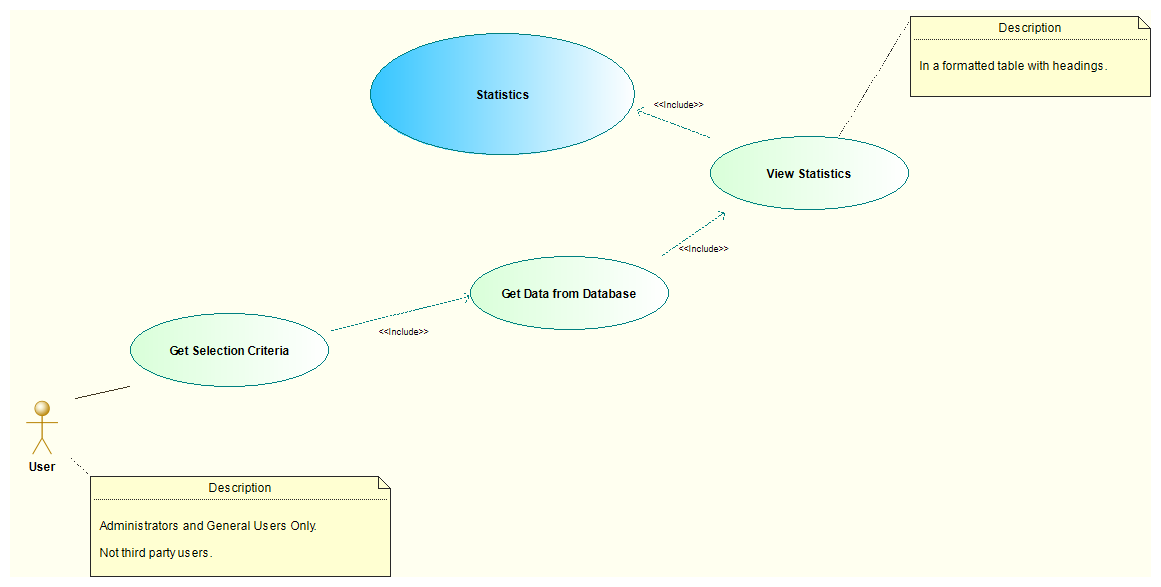
\includegraphics[width=\linewidth]{statistics/Statistics}}}